%%
%% Copyright 2007, 2008, 2009 Elsevier Ltd
%%
%% This file is part of the 'Elsarticle Bundle'.
%% ---------------------------------------------
%%
%% It may be distributed under the conditions of the LaTeX Project Public
%% License, either version 1.2 of this license or (at your option) any
%% later version.  The latest version of this license is in
%%    http://www.latex-project.org/lppl.txt
%% and version 1.2 or later is part of all distributions of LaTeX
%% version 1999/12/01 or later.
%%
%% The list of all files belonging to the 'Elsarticle Bundle' is
%% given in the file `manifest.txt'.
%%

%% Template article for Elsevier's document class `elsarticle'
%% with numbered style bibliographic references
%% SP 2008/03/01
%%
%%
%%
%% $Id: elsarticle-template-num.tex 4 2009-10-24 08:22:58Z rishi $
%%
%%
\documentclass[preprint,12pt]{elsarticle}
\usepackage{algorithm}
\usepackage{algpseudocode}
%% Use the option review to obtain double line spacing
%% \documentclass[preprint,review,12pt]{elsarticle}

%% Use the options 1p,twocolumn; 3p; 3p,twocolumn; 5p; or 5p,twocolumn
%% for a journal layout:
%% \documentclass[final,1p,times]{elsarticle}
%% \documentclass[final,1p,times,twocolumn]{elsarticle}
%% \documentclass[final,3p,times]{elsarticle}
%% \documentclass[final,3p,times,twocolumn]{elsarticle}
%% \documentclass[final,5p,times]{elsarticle}
%% \documentclass[final,5p,times,twocolumn]{elsarticle}

%% if you use PostScript figures in your article
%% use the graphics package for simple commands
%% \usepackage{graphics}
%% or use the graphicx package for more complicated commands
%% \usepackage{graphicx}
%% or use the epsfig package if you prefer to use the old commands
%% \usepackage{epsfig}

%% The amssymb package provides various useful mathematical symbols
\usepackage{amssymb}
\usepackage{amsmath}
%% The amsthm package provides extended theorem environments
%%\usepackage{amsthm}

%% The lineno packages adds line numbers. Start line numbering with
%% \begin{linenumbers}, end it with \end{linenumbers}. Or switch it on
%% for the whole article with \linenumbers after \end{frontmatter}.
%% \usepackage{lineno}

%% natbib.sty is loaded by default. However, natbib options can be
%% provided with \biboptions{...} command. Following options are
%% valid:

%%   round  -  round parentheses are used (default)
%%   square -  square brackets are used   [option]
%%   curly  -  curly braces are used      {option}
%%   angle  -  angle brackets are used    <option>
%%   semicolon  -  multiple citations separated by semi-colon
%%   colon  - same as semicolon, an earlier confusion
%%   comma  -  separated by comma
%%   numbers-  selects numerical citations
%%   super  -  numerical citations as superscripts
%%   sort   -  sorts multiple citations according to order in ref. list
%%   sort&compress   -  like sort, but also compresses numerical citations
%%   compress - compresses without sorting
%%
%% \biboptions{comma,round}

% \biboptions{}


\journal{Computer Aided Geometric Design}

\begin{document}

\begin{frontmatter}

%% Title, authors and addresses

%% use the tnoteref command within \title for footnotes;
%% use the tnotetext command for the associated footnote;
%% use the fnref command within \author or \address for footnotes;
%% use the fntext command for the associated footnote;
%% use the corref command within \author for corresponding author footnotes;
%% use the cortext command for the associated footnote;
%% use the ead command for the email address,
%% and the form \ead[url] for the home page:
%%
%% \title{Title\tnoteref{label1}}
%% \tnotetext[label1]{}
%% \author{Name\corref{cor1}\fnref{label2}}
%% \ead{email address}
%% \ead[url]{home page}
%% \fntext[label2]{}
%% \cortext[cor1]{}
%% \address{Address\fnref{label3}}
%% \fntext[label3]{}

\title{Automated Edge Grid Generation Based on Arc Length Optimization}

%% use optional labels to link authors explicitly to addresses:
%% \author[label1,label2]{<author name>}
%% \address[label1]{<address>}
%% \address[label2]{<address>}

\author[David]{David McLaurin}
\author[Suzanne]{Suzanne Shontz}
\address[David]{Mississippi State Univesity, Starkville, MS}
\address[Suzanne]{Mississippi State Univesity, Starkville, MS}

\begin{abstract}
Computational design and analysis has become a fundamental part of industry and academia for use in research, development, and manufacturing. In general, the accuracy of a computational analysis depends heavily on the fidelity of the computational representation of a real-world object or phenomenon. Most mesh generation strategies focus on element quality--with the justification being that downstream applications require high quality geometries in order to achieve a desired level of accuracy. However, element quality should be secondary to accurately representing the underly physical object or phenomenon. This work seeks to improve the process of creating a computational model of an object of interest by accelerating the process of mesh generation by reducing the need for (often) manual intervention. This acceleration will be accomplished by automatically generating \textit{optimal} discretizations of curves by minimizing the \textit{arc-length deficit}. Methods were developed to generate optimal discretizations through local or global optimization. Results are presented showing the robustness and accuracy of the developed methods along with a presentation of how to implement the developed methods into an existing mesh generator.
\end{abstract}

\begin{keyword}
%% keywords here, in the form: keyword \sep keyword

%% MSC codes here, in the form: \MSC code \sep code
%% or \MSC[2008] code \sep code (2000 is the default)
mesh \sep optimal \sep adaptive \sep automated \sep grid
\end{keyword}

\end{frontmatter}

%%
%% Start line numbering here if you want
%%
% \linenumbers

%% main text

\section{Introduction}Computational design and analysis has become a fundamental part of industry and academia for use in research, development, and manufacturing. In general, the accuracy of a computational analysis depends heavily on the fidelity of the computational representation of a real-world object or phenomenon. However, the task of creating high fidelity models of an actual geometry can be time-consuming--sometimes consuming up to seventy-five percent of the time required to produce a solution \cite{bischoff05}. This work seeks to improve the process of creating a computational model of an object of interest by accelerating the process of mesh generation. Below in Figure-\ref{GridGenerationProcess} an example of a mesh generation hierarchy can be seen. In general, a valid volume grid (three-dimensional) is bounded by surface grids (two-dimensional); and surface grids are bounded by edge-grids (one-dimensional). At the start of the grid generation hierarchy are point spacing values at the end points of analytical or parametric curves—which bound the edge-grids. In most cases, volume-grid generation is a highly automated procedure—once the bounding surfaces are generated. The same generalization can be made for surface-grids and edge-grids. Algorithms that use automated point creation/insertion for mesh generation of one-, two-, and three-dimensional geometries are ubiquitous [REFERENCES, CUBIT, Delaunay, AFLR]. However the authors are only aware of one such automated scheme for setting point spacing values for more automated mesh generation \cite{mclaurin12}.\\

\begin{figure}[h!]
 \center{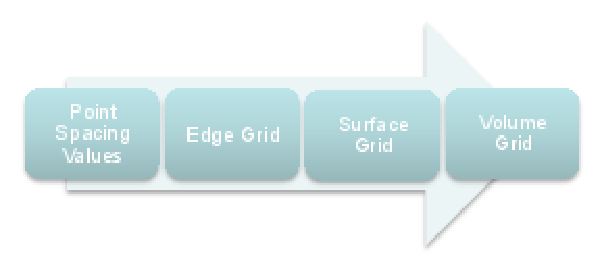
\includegraphics[width=0.8\textwidth]
  {Figures/GridGenProcess.eps}}
 \caption{\label{GridGenerationProcess} Specified point spacings and final point distribution for a surface edge \cite{thompson98}}
\end{figure}

The computation involved with edge-grid generation is trivial when compared to volume-grid generation—even with high-order NURBS curves. However, the point spacing values at the end points of curves have to be set manually in order to satisfy a desired length scale. This manual process is time consuming. If geometry repair (gluing, trimming, etc…) is not considered, the amount of user input required to generate a volume grid can be concentrated on the lowest levels of the grid generation hierarchy. In addition, if the edge-grids are not generated appropriately then the errors present there, such as overly dense or sparse spacing, will be propagated up the hierarchy and be present in each subsequent higher-dimensional entity. In order to accelerate the process of generating edge grids, some degree of automation is needed to help deal with common issues associated with undesirable edge-grids.

The proposed algorithm is a general-use method that can be applied to any ``digital curve'' regardless of its representation. This is due to every step being developed without the use of derivatives. Most other methods operate on a specific type of curve, such as NURBS or B-splines, and use the specific information available for the type of curve in use. While in the field of CAD NURBS curves are the de-facto standard, in other fields, such as pattern-recognition, other types of digital curves, such as parametric, are more common[REFERENCES]. T-splines are also becoming more popular in applications such as isogeometric analysis [REFERENCES, Thomas Hughes]. Therefore a general algorithm that does not require derivative information to generate a suitable edge grid was developed. A result of not using derivatives is that each step in the algorithm is robust to large changes in derivatives or curves that are not ``well behaved''---highly oscillatory for instance.

The justification for the development of these methods lies in the need for an automated way of setting point spacing values on curves. This process can only be automated if some way of judging ``how well'' an edge grid represents a curve is present. To this end, two related methods of generating edge grids through constrained optimization are detailed below. Further discussion of element quality, robustness, and a framework for implementing the information associated with an optimal edge grid into an existing grid generator is also presented. Generating edge grids in a more automated fashion accelerates the process of surface grid generation---and ultimately volume grid generation. Using the detailed methods, or any other automated method for setting point spacings does not change the number of steps required for grid generation. However, it does reduce the number of manual steps involved in starting the process.

\section{Related Work}
In general, grid generation is a name for any process that creates a grid.  For example, the advancing-front algorithm advances boundaries into space to generate a grid \cite{lohner88}.  Other methods generate grids from iterative refinement or enrichment from initial, coarse configurations[cite].  Usually the benchmark for separating the two methods, generation and refinement, are the prioritization of grid quality and grid accuracy (both of these issues will be addressed later).  From a standard text \cite{thompson98}: One dimensional grids, or edge grids, \begin{quotation} \noindent ``...are created using a one-dimensional version of the standard grid generation procedure.  This ensures that point distribution and growth rates are fully compatible for optimal final grid quality.  For each edge or segment the point spacing is specified at both ends…edge grid generation is then used to produce the point distribution...'' \end{quotation} An example of this can be seen below in Figure-\ref{EdgeGrid_HandbookOfGridGeneration} where the point spacing distributions are df1 and df2.

\begin{figure}[h!]
  \center{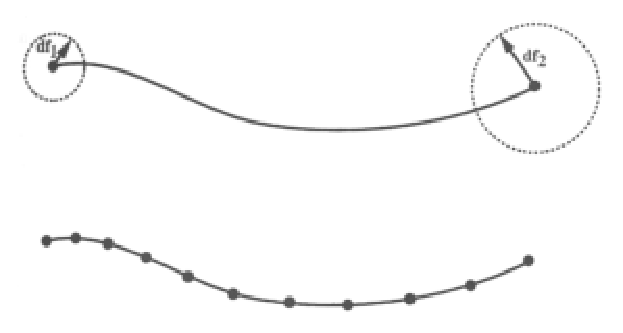
\includegraphics[width=0.8\textwidth]
    {Figures/EdgeGrid_HandbookOfGridGeneration.eps}}
  \caption{\label{EdgeGrid_HandbookOfGridGeneration} Caption}
\end{figure}

\noindent In the example above, the edge grid generation process produces good quality grids from the combination of geometric growth rates and smoothing.  However, the process requires input: point spacing values.  If the point spacing values are not appropriate then the geometry can be under and/or over sampled for the intended use.  That fact is not an indictment of the grid generation process, but instead implies that the final grid is heavily dependent on the inputs.  In addition, if some way of controlling the point spacing in the middle of a curve is not present, then more points could be wasted/omitted in an attempt to accurately represent geometry.

Instead of setting appropriate point spacing values and using common grid generation techniques, other efforts have gone into creating a locally or globally ``optimal'' edge grid.  Many names have been assigned to this particular task, but the underlying goal is very similar—represent a curve as accurately as possible—whatever that means for each application.  For example, \cite{laug04} first linearized the interface between curves in order to simplify the process of generating edge grids and surface grids on topologically adjacent patches.  Other ``geometry aware'' or ``curvature based'' approaches have been developed.  One such application is for discretizing curves for use in level set methods \cite{macklin06}.  Others include energy minimization \cite{hofer04}, curvature minimization \cite{zehiry10}, and angle minimization \cite{ebeida10}.

\section{Discretization Error}
The accuracy, or discretization error, of a piecewise, linear representation ($discretization$) of an analytical curve ($curve$) in $R^3$ can be defined in many ways depending on the intended application.  The error associated with the $discretization$ is discussed in terms of the ``deviation'' from the $curve$—most often quantified by calculating or approximating the distance from the $curve$ for each linear segment in the $discretization$, or the area of the ruled surface between a curve-piece and the segment representing that part of the $curve$.  Another way of quantifying the error associated with a $discretization$ would be to consider how well it approximates the arc length of the $curve$ it represents.  In general the arc length is not known a priori, but depending on the underlying representation it can be calculated exactly (parametric or analytical) or can be estimated (Bezier).  One of the goals of this method was to be “general” in that it should be independent of the underlying geometric representation.  Therefore a method that requires the arc-length of the underlying geometry violates the aforementioned concept of “generality” and restricts the applications for which the proposed method could be applied.  Some other way of determining/generating an edge grid based on arc length is needed.  This process will be detailed later.

Arc-length convergence of a $discretization$ is a sufficient condition for other schemes of edge grid generation/refinement.  That is: if the difference between the arc length of the $curve$ and the sum of the segments in the $discretization$ approaches zero then that is sufficient to conclude that the distance between the $discretization$ and the $curve$ is also approaching zero, also the angles between segments approaches 180 degrees.  However, the converse of that statement is not true.  The pathological case of a highly oscillatory, low amplitude $curve$ approximated by two straight lines shows that a $discretization$ of a $curve$ can have a small ``deviation'' or angles between segments but be a poor estimate for arc length.[PICTURE]  Another pathological case is a ``non-convex'' $curve$ where the parameterization goes well ``outside'' of the segment.

\section{Discrete Curvature Approximation}
The concept of ``deviation'' as defined above is relatively straightforward and intuitive. However, another related way of describing ``how well'' a \textit{discretization} represents a \textit{curve} is the degree to which the discrete representation approximates curvature—where curvature is defined as the amount of ``bend'' in a \textit{curve} or surface, or ``how much'' a \textit{curve} or surface ``differs'' from a straight line or plane (words in quotes are subject to gradation). First, however, curvature must be defined in such a way that a discrete approximation is meaningful and appropriate. In relevant literature there are many ways to estimate curvature \cite{hermann07}. Some of it bears repeating because it is germane to what is being discussed here: Consider the following planar \textit{curve}, C, at point P. At a given point P there exists an osculating circle, O, of radius r such that the circle has the same tangent as the \textit{curve} C as well as the same radius of curvature \cite{gray97}. \\

\begin{figure}[h!]
  \center{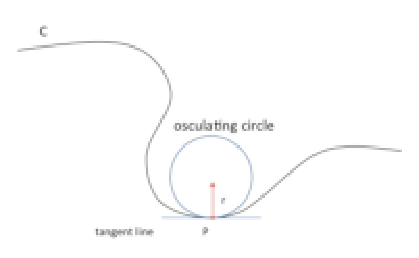
\includegraphics
    {Figures/OsculatingCircle.eps}}
  \caption{\label{OsculatingCircle} Osculating Circle of a Planar Curve}
\end{figure}

\noindent Just as the tangent line is the line best approximating a \textit{curve} at a point, the osculating circle is the best circle that approximates the \textit{curve} a point. Ignoring degenerate \textit{curve}s such as straight lines, the osculating circle of a given \textit{curve} at a given point is unique \cite{gray97}. The radius, r, of the osculating circle at a given point on a \textit{curve} is equal to the radius of curvature, R, which is the reciprocal of curvature, $\kappa$--sometimes called the ``first curvature'' \cite{kreyszig91}. For a two-dimensional \textit{curve} of the form $y=f(x)$, the equation for curvature is:
\[ 
R=\frac{1}{\kappa} \textnormal{ , where } \kappa=\frac{\frac{d^2y}{dx^2}}{[1+\frac{dy}{dx}^2 ]^\frac{3}{2}} 
\]
\noindent This quantity, kappa, necessarily includes the calculating of derivatives which, depending on the representation of the underlying geometrical description, could be relatively costly. Therefore, this is avoided by defining this radius of curvature on a segment or at a point in the \textit{discretization} without the use of derivatives. This is discussed in the following paragraphs.

A value of curvature can be calculated for each edge in the \textit{discretization} by considering the corresponding osculating circle on a given edge. The osculating circle here (circle, Figure 2) can be approximated by considering the circumscribed circle (circumcircle) \cite{casey1888} defined by the two end points of the edge, P0 and P1, and a point, P, between them in the \textit{curve} parameterization—the radius of the circumcircle will be referred to as the discrete radius of curvature.

\begin{figure}[h!]
  \center{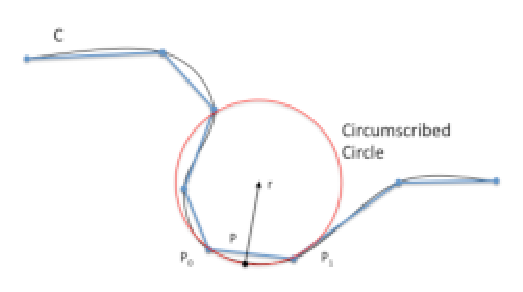
\includegraphics
    {Figures/CircumscribedCircle.eps}}
  \caption{\label{CircumscribedCircle} Caption}
\end{figure}

\noindent The method of choosing this point, P, and its importance to an accurate mesh refinement will be detailed later. This definition/approximation of the radius of curvature of the \textit{curve}/\textit{discretization} is useful for this application, but exhibits scale-dependence. The discrete radius of curvature alone is not sufficient to determine how well a segment approximates the curvature. The discrete radius of curvature must be given some context. In other words: it must be compared to the local feature size in order to determine if the segment is an accurate representation. Another problem with comparing the radius of curvature and the discrete radius of curvature is that as the \textit{discretization} becomes more refined the discrete radius of curvature approaches infinity and therefore diverges from the analytical value at that point. Stated another way, as the sum of the length of the segments in the \textit{discretization} converges to the actual length of the \textit{curve}, the discrete radius of curvature of each segment approaches infinity. Therefore, a quantity is needed that is scale-independent that converges to a computer-representable value as the \textit{discretization} becomes more refined.
Proof: Consider a circular segment--which represents the \textit{curve} (\textit{s}), the corresponding chord--which represents a segment in the \textit{discretization}--(\textit{a}), and saggitta--which represents the ``deviation'' of the segment away from the \textit{curve} (\textit{h}) in Figure-\ref{CircleGeometry} :
\begin{figure}
  \center{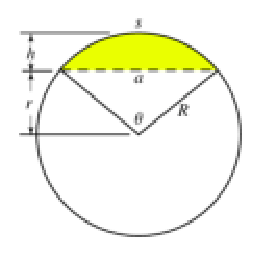
\includegraphics
    {Figures/CircleGeometry.eps}}
  \caption{\label{CircleGeometry} Caption}
\end{figure}

As the length of a approaches the length of s, the length of h goes to zero, therefore the radius of the circle, R, goes to infinity.\\
(1) $a=\sqrt{R^2+r^2}=2*\sqrt{(h*(2*R-h)}$ \hspace{2pt} which rearranged yields: \\
(2) $R=\frac{(\frac{a}{2})^2*\frac{1}{h}+h}{2}=
\frac{a^2+4*h^2}{8*h}=\frac{a^2}{8*h}+\frac{h}{2}$\\
(3) $lim_{h\to0}(\frac{a^2}{(8*h)}+\frac{h}{2})=\infty$ \\

Given the aforementioned proof, if the discrete curvature radius is divided by the length of the corresponding segment on the \textit{curve}, then it’s value approaches zero. This is a scale independent measure that converges to a computer representable number as the \textit{discretization} approaches the length of the \textit{curve}. The parameter is known as the curvature ratio. It is an intuitive measure that relates ``how far'' the \textit{curve} deviates from the segment that is representing it as the ratio of those lengths. Consider a point on a \textit{curve} between two endpoints of a segment of a \textit{discretization}, as seen in Figure-\ref{CurvatureRatio}. The length of the segment, $L_i$, is the distance from $P_0$ to $P_1$. The perpendicular distance between the point on the \textit{curve} between the end points and the segment is $L_c$. The three points define a Curvature Ratio through the ratio of $L_c$ to $L_i$.

\begin{figure}[h!]
  \center{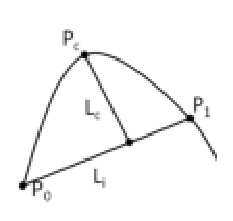
\includegraphics
    {Figures/CurvatureRatio.eps}}
  \caption{\label{CurvatureRatio} $Curvature Ratio=  \frac{L_c}{L_i}$ \cite{mclaurin10}}
\end{figure}

(pattern recognition is a field that has some research in this area)

\section{Refinement via Maximum Curvature Ratio/Deviation}
One could, for instance, find the maximum value for curvature ratio on the segment to determine whether or not to further subdivide the segment.  This is an example of “deviation-based” refinement.  For a given segment, the maximum curvature ratio is found where the perpendicular distance between the segment and the curve is maximum.  This might not correspond to the point where the combined arc-length of the two new segments is maximally different from the current configuration.  For instance consider the triangle, (\textit{A}, \textit{B}, \textit{C}) with sides of length following the Pythagorean triple (5,12,13) and therefore perimeter of 30.

\begin{figure}[h!]
  \center{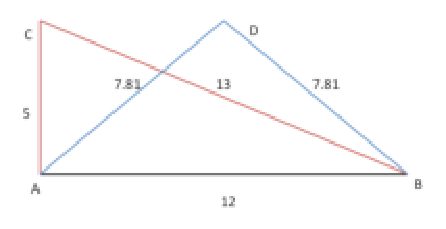
\includegraphics
    {Figures/CurvatureRatioTriangles.eps}}
  \caption{\label{CurvatureRatioTriangles} Caption}
\end{figure}

\noindent Additionally consider the triangle (\textit{A}, \textit{B}, \textit{D}) formed with the same base (12) and height (5) as the other triangle.  The perimeter of this triangle, (\textit{A}, \textit{B}, \textit{D}) is 27.62. Using point \textit{C} to increases the length of the segment locally by 150\%, while using point \textit{D} increases the length of the segment by 130.1\%.  Both of these triangles have the same Curvature Ratio since their bases and heights are identical.  However, as shown the perimeter can vary a not-insignificant amount without changing the Curvature Ratio of a segment.  Therefore, the Curvature Ratio is not sufficient to determine whether or not the arc-length of the discretization is approaching that of the curve—only that the distance between the discretization and the curve is approaching some value locally.  Using only the Curvature Ratio, the choice between point \textit{C} and \textit{D} in Figure-\ref{CurvatureRatioTriangles} are equal.  The potential error would get worse if the point \textit{C} were moved further left--demonstrating that the Curvature Ratio is not always a good indicator of discretization accuracy for curves that aren’t ``well-behaved'' between discrete segments.

\section{Refinement via Arc-Length Deficit}
Mentioned above, a way of determining ``how well'' a discretization approximates a curve was to consider the difference between arc lengths.  This posed another way as ``how well'' it captures curvature.  Locally, it is important for each segment in the discretization to represent the local geometry present in the curve.  If a segment is to be subdivided in order to improve the discretization, then it should be subdivided in a way that is most effective/efficient locally.  Also, if the purpose of the refinement process is to minimize the actual arc length minus the discrete arc length, then an optimization problem can be formed where an objective function is minimized as the combined length of the segments in the discretization approach that of the curve.

Let $C(u)$ be a parameterized curve, and $D$ be a discretization of the curve comprised of a number, $n_t$, of points, $P_i : i \in \{1,...n_t\}$, and segmenets, $S_j : j \in \{1,...,(n_t-1)\}$. Segment $S_j$ is defined by two successive parameterization values, $u_j$ and $u_{j+1}$. If $L(S)$ is a function that calculates the length of a segment  in $(x,y,z)$ space then the optimization problem can be stated as:
\begin{equation}
\begin{aligned}
& \underset{u_i}{\text{minimize}}
&& O=-\sum{_{j=2}^{n_t-1}L_j} \\
& \text{subject to}
&& (u_1 = a, u_1<u_2, u_2<u_3,..., u_{n_t-2}< u_{n_t-1}, u_{n_t} = b)
\end{aligned}
\end{equation}

\noindent The resulting optimization problem is linear[PROVE] and a variety of standard methods (subsets of linear programming) could be used to obtain a solution.  The analysis and calculation are straightforward for a defined number of interior points.  For this method to be practical, however, one would have to know a priori how many points on the interior of the curve were desired.  Either that, or repeatedly solve the optimization problem with an increasing number of interior points until the combined length of the segments in the discretization converged to a desirable tolerance.

One could not formally include the number of interior points into the definition of the optimization problem because the number of interior points could only be given a lower bound, 0.  An upper bound is needed due to the fact that the (not an) ``optimal'' discretization (as defined above) without an upper bound contains an infinite amount of interior points.  In order to impose an upper bound, one could constrain the problem further with a lower bound on the distance between points:

a user-defined minimum tolerance, $e$, is easily worked into the set of constraints, where $P_i$ represents a point in non-parametrized, $(x,y,z)$, space: \\
$(P_1 = \alpha, P_1+e <= P_2, P_2+e <= P_3, … , P_{n_t-2}+ e <= P_{n_t-1}, P_{n_t} = \beta)$ \\

\noindent An upper bound on the distance between points could also be implemented, where $P_i$ represents a point in non-parameterized, $(x,y,z)$, space:

a user-defined maximum tolerance, $m$, is easily worked in as an additional set of constraints: \\
$(P_1 = \alpha, P_1+m >= P_2, P_2+m >= P_3, … , P_{n_t-2}+ m >= P_{n_t-1}, P_{n_t} = \beta)$ \\

\noindent The definition of a lower and upper bounds for the distance between points implicitly defines an upper and lower bound for the number of interior points.  The implicit definition would be in the form of an over-constrained problem where solutions did not exist for too many or too few points.  For instance, too many points could not satisfy the minimum-distance set of constraints and too few points could not satisfy the maximum-distance set of constraints.  However, explicitly determining these bounds for $n_t$ would prove difficult.  It could, for example, involve repeatedly sampling the curve to determine the maximum number of e-length segments and the minimum number of m-length segments.  This would be possible, but inefficient.  Another option is to estimate the number of points needed \cite{cuilliere97}.  However, if $n_t$ is to be estimated then the discretization is not guaranteed to optimal. Therefore, the conclusion is that a global optimization problem, while possible, is not very practical in this case.  One of the aims of this work is to accelerate the generation of suitable grids for simulation; and moving the bottleneck for grid generation to the lowest level in the grid generation hierarchy just increases the amount of time required to generate a grid.  The above method does however represents a solution to the problem of generating automated, optimal edge-grids.

Others have attempted dynamic programming methods for generating ``optimal'' discretizations for digital curves \cite{horng02}.  However, in general this should prove no more effective than any of the approaches mentioned above.  It is true that the problem of generating a discretization to accurately represent a curve exhibits optimal substructure—which is defined where ``...an optimal solution can be constructed efficiently from optimal solutions to its subproblems.'' \cite{cormen01}  However, the number of distinct subproblems available that represent an optimal solution at a defined error bound can be infinite.  Therefore, instead of trying to find an optimal number of nodes required for an optimal discretization (which seems very inefficient), the proposed algorithm will use a divide-and-conquer (recursive) approach to generating an ideal discretization relative to a given tolerance.  The combination of the optimized segments represents an optimal discretization for the entire curve.

This would generate an optimal solution using two segments to represent the entire curve—which can be stated another way as maximizing the perimeter of the triangle formed by the existing segment and the two new segments.  Consider that the red triangle in Figure-\ref{CurvatureRatioTriangles} has a larger perimeter than the blue triangle; therefore the red triangle would be considered ``more optimal.'' The above optimization problem could then be applied recursively to each new segment with $n_t=3$.  This process breaks the task of optimizing a discretization for an entire curve into optimizing a simple discretization for smaller section of the curve with the following algorithm.  The optimization algorithm described above with $n_t=3$ for a given segment is:

\begin{algorithm}
\caption{Optimization Algorithm with $n_t=3$}\label{localoptimize}
\begin{algorithmic}[1]
\State $n_t = 3$
\State $u_i : i \in \{1,2,3\}$
\State $u_1 $ and $u_3$ define the segment $S_{1,3}$
\Procedure{Local Optimization}{$S_{1,3}$}
  \State $L(S_{1,3}) =\textnormal{ length of segment}$
  \State Place interior point $u_2$ to maximize $L(S_{1,2})+L(S_{1,3})$ within $tolerance$
\EndProcedure
\end{algorithmic}
\end{algorithm}

The would be applied for each segment in the discretization by:

\begin{algorithm}
\caption{Optimization Algorithm for Discretization}
\begin{algorithmic}
  \State $D(S_j) : j \in {1}$
  \State push $S_1$ into $list$ \Comment{$list$ is $queue$ if breadth-first, $stack$ if depth-first}
  \While{$list$ is not empty}
    \State pop $S_j$ from $list$
    \If {$S_i$ is optimal}
      \State do nothing
    \Else
      \State optimize $S_j$ with Algorithm: \ref{localoptimize}
      \State push $S_{i,i+\frac{1}{2}}$ into $list$
      \State push $S_{i+\frac{1}{2},i+1}$ into $list$
    \EndIf
  \EndWhile
\end{algorithmic}
\end{algorithm}

The above algorithm is straightforward and is often referred to as adaptive refinement or enrichment (see above).  Also, since the discretization of the curve exhibits optimal substructure, the starting point to the optimization algorithm and the method of refinement or enrichment are irrelevant to the extent to which they prevent an optimal solution from being generated.  However, the initial discretization and choice of refinement strategy/order of application obviously con
tributes to the efficiency of the algorithm.

Now to define the optimization part of the above algorithm:  Divide and conquer can be considered to be based on multi-branched recursion.  The objects to be constructed at the end of the recursion are the smallest set of segments that approximates the arc-length of the curve to a defined precision.  This is not quantifiable without the a priori knowledge of the arc-length of the curve.  As discussed above, calculating the length of a curve for this application is impractical.  So how can the ``goodness'' of a discretization be measured?  At each step, the discretization will be refined on each segment by locally optimizing an objective function analogous to the one developed above.  In order to minimize each segment’s objective function, arc length deficit ($ALD$), then a point $P$ has to be placed on the curve between the segment such that the new sum of the arc lengths is changed maximally.  Since this entire project is to be done without calculating derivatives (see reasons above), the optimization scheme chosen here is not given access to derivative information either.  Since the optimization function is a non-negative planar curve, $(O: C \rightarrow ALD)$, any line-searching method of optimization could be used.  However, the method cannot have any requirements on differentiability due to the possibility that the derivative of $O$ could be discontinuous if the curve passed through the segment.  Consider the function $f(x)=x^3-3x^2-144x+432$, plotted in red in Figure-\ref{OptimizationFunctionExample} with the blue line representing the corresponding segment.  The middle figure shows the graph of the optimization function (as defined above).  Notice at the root, 3, the curve crosses the x-axis and the derivative of the optimization function does not exist.  This can be seen right Figure-\ref{OptimizationFunctionExample} which is a plot of the derivative of the optimization curve.  The red line represents the limit approaching from $-\infty$ and the blue line represents the limit approaching from $+\infty$.

\begin{figure}[h!]
  \center{
    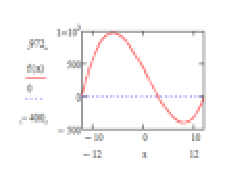
\includegraphics{Figures/CurvePlot.eps}
    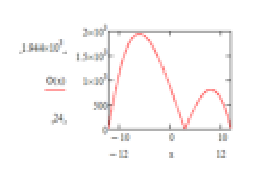
\includegraphics{Figures/OFunctionPlot.eps}
    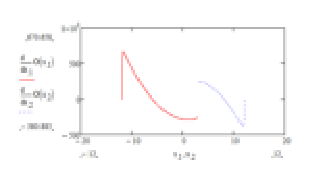
\includegraphics{Figures/ODerivativePlot.eps}
  }
  \caption{\label{OptimizationFunctionExample} Caption}
\end{figure}

The Golden-Section Search Method is implemented here since it meets all of the above criteria and has the possibility to converge superlinearly \cite{brent73}--unlike the bisection method.  If the length of each segment locally approaches the portion of the curve it represents (local objective function is minimized), then the global length of the discretization approaches the global length of the curve (a restatement of the property of optimal substructure).  Also, since the optimization algorithm for each segment is only concerned about the portion of the curve it represents, then this method exhibits scale-independence—which was one of the requirements for the algorithm.

Recursive algorithms require stopping criteria.  In this case the stopping criteria should not permit the method to infinitely subdivide the curve.  For instance, the aforementioned minimum and maximum segment lengths can be used (and were implemented here).  Even though using a minimum edge length would prevent the infinite subdivision of the curve, another criteria is needed such that the minimum segment length is not needed to satisfy the criteria.  This stopping criterion could be in the form of a delta-segment length.  That is, if the new segments’ combined length is below a defined fraction larger than the existing segment then it should not be subdivided.  This is a ``pure-greedy'' method of subdivision, in that it does not consider the rest of the ``solution'' when deciding to stop.  One problem with this set of stopping criterion is immediately apparent: the ``large'' segments could potentially not be subdivided because locally it is not justified—even if the subdivision of that large segment would cause a global change in the length of the curve that is significant.  This value, global delta-segment, would have to be smaller than the one used locally for each segment; otherwise it would have no effect.  Therefore, an additional criterion is needed to determine if a segment should be subdivided: if the total change in length of the discretization would be changed by a defined fraction then it should be subdivided.  The addition of this last subdivision criterion makes the method ``less-greedy''.  This set, minimum segment length, maximum segment length, local delta-segment, and global delta-segment define a robust, minimum set of criterion needed for generating an optimum solution to the problem of representing a curve via arc-length deficit.

\section{Error Bounds}
Now that the problem has been stated and a solution has been formulated, error bounds for the proposed algorithm should be discussed.  Since the optimization function for each curve is not given access to derivative information, it is conceivable that it would not find the optimal value and instead converge to a local minimum.  However, the problem of escaping local minima is common to all optimization problems.  The addition of the conditional that states: ``refine a segment if the refinement changes the length of the entire discretization by more than an epsilon'' was deliberately included to lessen the chance that a segment would not be refined when it was prudent to do so.  If the method succeeds in finding the global minimum for each segment, then the error bound will be on the order of the delta-segment.  However, when the method fails to do so, or chooses a local minimum instead, there is no formal way to express the error as a function of arc-length-deficit--since there is no information about what the global minimum might be (without explicitly calculating the length of the curve/segment).  Therefore, the error can only be quantified for when the method has succeeded in finding the minimum for each segment.

        Arc-length-deficit is a single-value function on the curve.  The obvious problem with this single-valued function is that the actual arc-length of the curve is never known and can therefore not be compared to the arc-length of the segments.  How then can we quantify the error?  The error bounds could be detailed for unimodal pieces of the curve--those where the ALD function has one peak. However, for segments that do not have a unimodal distribution of the ALD function on the local curve segment, the error estimation is not straightforward.  It is no longer possible to determine what the bound for the arc-length-deficit error is.  However, we can state some observations about the geometry related to these configurations:

Assume that the optimization function on a general segment found the global minimum, i.e. maximized the change in edge-length for the new combined segments, for the segment and corresponding curve piece.  With the given geometry, an ellipsoid can be formed with the endpoints of the segment, $F_1$ and $F_2$, as the foci and the semi-major and semi-minor axes are defined implicitly by the new segments connecting the new point with the endpoints of the current segment, $r_1$ and $r_2$.  ``An ellipse is a curve that is the locus of all points in the plane the sum of whose distances $r_1$ and $r_2$ from two fixed points $F_1$ and $F_2$ (the foci) separated by a distance of $2c$ is a given positive constant $2a$'' \cite{weissteine}.  With the above assumption and definition, the entirety of the curve represented by the segment must lie within the prolate spheroid  formed by the geometry below in Figure-\ref{EllipseGeometry}.

\begin{figure}[h!]
  \center{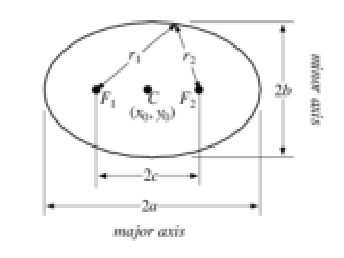
\includegraphics
    {Figures/EllipseGeometry.eps}}
  \caption{\label{EllipseGeometry} Caption}
\end{figure}

Proof: If the perimeter is maximized keeping $2c$ a constant, $(r_1 + r_2)$ is maximized \textit{because} $2c$ is a constant.  Maximizing $(r_1+r_2)$ maximizes a from the following relation with $2c$ being constant: $r_1 + r_2 = 2a$.  Combining the following relation, $b^2 = a^2 + c^2$, with the area of the ellipse, $A = \pi * a * b$, yields $A=\pi^{2}*a^{2}(a^{2} - c^2)$.  If $c$ is a constant and $a$ is maximized, then the maximal area is obtained from maximal $(r_1+r_2)$.  Which means the curve must be inside of the spheroid defined by the ellipse.  If the curve is not inside the spheroid then there is a point on the curve such that $(r_1+r_2)$ is larger and therefore the area is larger and therefore the volume is larger which means that $(r_1+r_2)$ was not maximized.

        Observe that there was no mention of the length of the curve inside of the spheroid, or the ruled area that the segment and curve could define.  This is because there is no way this information can be known (without explicitly calculating the length of the curve/segment).  It is unfortunate that there is no way to quantify the discretization error of a curve except in terms of volume of the spheroids defined by each segment.  This is non-intuitive, but no more specificity is possible.  The volumes would also be scale-dependent and offer no insight into how well the discretization approximates the curve—without some context.
[stuff about ellipsoids and volume, proof of containing ellipse, etc…]

\section{Element Quality}
A topic that has not been discussed thus far is element quality.  Element quality is an intuitive measure for surface elements, e.g. triangles; but how to define quality for a line segment?  In this context, the notion of quality refers to the change in length between two topologically adjacent segments.  For the purposes of representing the curve to a desired tolerance, grid quality is not a concern.  However, for most applications the grid quality directly affects downstream uses, e.g. CFD, CEM, etc…  Therefore some discussion of this topic is warranted.  Grid quality in terms of edge grids is most often defined in terms of growth ratio, i.e. the length of a segment divided by the length of a topologically adjacent segment.  If the growth ratio strongly deviates from unity then the sizes of neighboring elements are not similar.  This will lead to a large disparity in the size of surface elements generated from them and that “error” in the form of a large growth ratio will be present in both the surface grid and volume grid in the vicinity of that portion of the edge grid.  This kind of disparate length scales can cause problems for finite element methods, finite volume methods, etc…

        Traditionally edge grids are generated with an a priori defined growth ratio along with other parameters that ensure that the grid has good quality.  A priori quality measures can be included in the constraints used in the global optimization procedure in a similar fashion to how the minimum and maximum edge lengths were included.  Post hoc methods for quality control could include some type of smoothing or (other type of) optimization [find more methods].  The author acknowledges that set of constraints grows very quickly in number with respect to the number of grid points—albeit linearly.  There is the set that defines the topology (1), the set that defines the minimum(2) and maximum(3) edge lengths, and now two more for minimum(4) and maximum(5) growth rates—for a total of five times the number of points.  For the local procedure, minimum and maximum growth rates could be include by splitting an edge if the growth rate is too large or small.

        One final method is to use the output from the developed methods, the “optimal” grid, as input for a grid generator—which presumably has strict quality control measures in place.  This would be accomplished by using the point spacing values present at the end points of the discretization at the end points of the curve.  The resulting edge grid from the grid generator could then be analyzed for the purpose of determining how far it deviates from “optimality” in the interior of the curve.  For instance, given a node on a generated edge grid, $x_i$, the corresponding parameterized value of $u_i$ could be found.  A point spacing value could be calculated at $u_i$ and compared to an interpolated value on the “optimal” edge grid.  If the values are found to be too disparate, then a point spacing source could be added to adjust the point spacing at that location.  The point spacing source would control the spacing during grid generation so that the generated edge grid would more closely resemble the spacing values present in the “optimal” grid while maintaining the quality typically associated with grid generators. In practice this usually leads to generated grids that are more fine than required by precision bounds due to the quality constraints imposed during grid generation.

\section{Results}

\section{Conclusions}

\section{Acknowledgements}

%% The Appendices part is started with the command \appendix;
%% appendix sections are then done as normal sections
%% \appendix

%% \section{}
%% \label{}

%% References
%%
%% Following citation commands can be used in the body text:
%% Usage of \cite is as follows:
%%   \cite{key}         ==>>  [#]
%%   \cite[chap. 2]{key} ==>> [#, chap. 2]
%%

%% References with bibTeX database:

\bibliographystyle{elsarticle-num}
\bibliography{References}

%% Authors are advised to submit their bibtex database files. They are
%% requested to list a bibtex style file in the manuscript if they do
%% not want to use elsarticle-num.bst.

%% References without bibTeX database:

% \begin{thebibliography}{00}

%% \bibitem must have the following form:
%%   \bibitem{key}...
%%

% \bibitem{}

% \end{thebibliography}


\end{document}

%%
%% End of file `elsarticle-template-num.tex'.
